\section*{Devil's Staircase}
\addcontentsline{toc}{subsection}{Devil's Staircase}
%%%
% Angabe
%%%
\subsection*{Angabe}
Ein Betrunkener versucht eine Treppe emporzusteigen -- dabei hat er so seine
Probleme, die folgendermassen beschrieben werden können. Dabei sei $p$ eine
reelle Zahl mit $0<p<1$, die als Wahrscheinlichkeit gedeutet wird\footnote{ $p$
steht nicht für ``Promille''! Je grösser $p$ ist, desto ``erfolgreicher'' ist
der Betrunkene.}

\begin{itemize}
 \item Die Treppe besteht aus den $k$ Zuständen (``Stufen'') $S_1 ,S_2, \ldots
	 S_k$. Der Betrunkene startet auf Stufe $S_1$.
 \item Mit jedem Schritt versucht er eine Stufe höher zu kommen, aber folgendes
	 passiert:
       	\begin{itemize}
	\item Wenn sich der Betrunkene auf Stufe $S_j$ mit $j<k$ befindet,
		schafft er es mit Wahrscheinlichkeit $p$ auf die Stufe
		$S_{j+1}$, aber mit Wahrscheinlichkeit $q=1-p$ fällt er auf die
		Stufe $S_1$ zurück.
	\item Wenn sich der Betrunkene auf Stufe $S_k$  befindet, fällt er mit
		Wahrscheinlichkeit $p+q=1$ ganz auf die Anfangsstufe $S_1$
		zurück.
	\end{itemize}
\end{itemize}
\begin{figure}[htbp] %  figure placement: here, top, bottom, or page
   \centering
   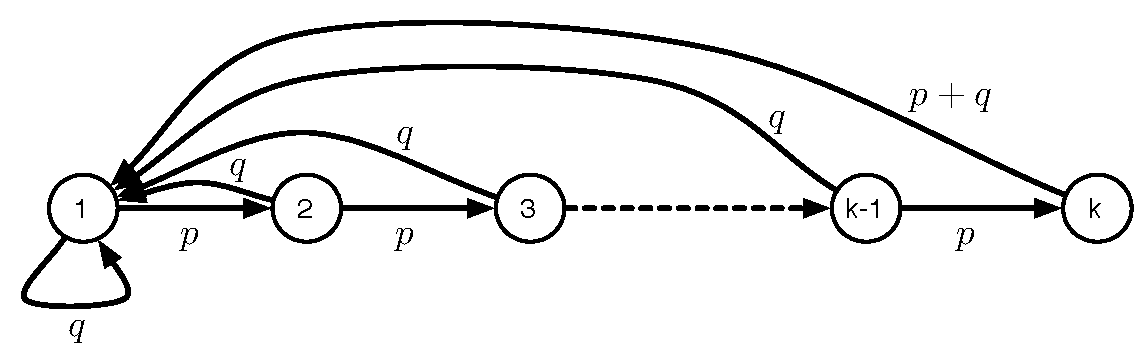
\includegraphics[width=4in]{graphics/devilsgraph.pdf} 
   %\caption{example caption}
   %\label{fig:example}
\end{figure}
Mit $T_k$ soll dieser ``Treppengraph'' bezeichnet werden''. Er hat also Knoten
(Zustände) $\{S_1,S_2,\ldots,S_k\}$ und die Kanten (Transitionen) wie
eingezeichnet.

Sie können diese grafische Darstellung 
\begin{itemize}
\item
entweder als einen endlichen Automaten (mit Startzustand $S_1$) interpretieren,
indem sie $p$ und $q$ als Symbole eines Eingabealphabets betrachten, oder
\item
als Markov-Kette betrachten, bei der die Transitionen zwischen den Zuständen
mit den Wahrscheinlichkeiten $p$ bzw. $q$ geschehen (und keine anderen als die
eingezeichneten vorkommen).
\end{itemize}

Betrachten sie zunächst die Automateninterpretation. Es bezeichne
$Ak_{i,j}^{(n)}$ die Anzahl der Pfade der Länge $n$ von $S_i$ nach $S_j$ in
$T_k$

\begin{flushenum}
\item Geben Sie explizit die Matrizen $Ak = \left[ Ak_{i,j}^{(1)} \right]$ für
	$k=2,3,4$ an und berechnen Sie deren charakteristisches Polynom.
	Welches sind die Eigenwerte?
\item Wie sehen die Matrizen $Ak$ allgemein aus, die das Geschehen in einem
	Schritt auf dieser ``Teufelsleiter'' beschreiben?\\ Zeigen Sie (z.B.
	per Induktion), dass
	\[
	\chi_{Ak}(z) = (z-2) \cdot \frac{z^k-1}{z-1}
	\]
	das charakteristische Polynom der Matrix $Ak$ ist.  Wo liegen die
	Eigenwerte der Matrix $Ak$ in der komplexen Ebene?  Machen Sie sich ein
	Bild davon!\footnote{ Bedenken Sie folgendes: das Polynom $X^k=1$ hat
	in $\mathbb{C}$ die $k$ Nullstellen $e^{2 \pi i (\ell/k)}$ für $0 \leq
	\ell < k$, genannt die (komplexen) $k$-ten Einheitswurzeln, die uns im
	Zusammenhang mit der Diskreten Fouriertransformation noch beschäftigen
	werden. Bezeichnet man mit $\omega_k$ die komplexe Zahl $e^{2 \pi i
	/k}= \cos (2 \pi/k) + i \cdot \sin(2 \pi/k)$, so sind die Nullstellen
	von $X^k=1$ gerade die Zahlen $\omega_k^\ell$ für $0 \leq \ell < k$,
	das sind die Teilungspunkte, wenn man den komplexen Einheitskreis der
	Länge $2 \pi$ in $k$ gleichlange Teile teilt, wobei $\omega_k^0=1$ ein
	Teilungspunkt ist.}
\item Betrachten Sie nun die Folgen
	\[
	\left(Ak_{1,j}^{(n)}\right)_{n \geq 0}~~\text{der Anzahlen der Pfade 
	der Länge $n$ von $S_1$ nach $S_j$ in $T_k$}
	\]
	Diese Folgen sind $C$-rekursiv und haben $\chi_{Ak}(z)$ als
	charakteristisches Polynom. \\
	Wie verhalten sich demnach die Folgen $\left(Ak_{1,j}^{(n)}\right)_{n \geq 0}$ asymptotisch 
	($n \rightarrow \infty$)? Ihre Antwort sollte die Form
	\[
	Ak_{1,j}^{(n)} \sim  \alpha_j \cdot \lambda^n
	\]
	haben. Dabei fragt sich
	\begin{itemize}
	\item Was ist $\lambda$ ? 
	\item Was ist $\alpha_j$ ?
	\end{itemize}
	Die Antwort auf die erste Frage ist einfach. \\
	Für die Antwort auf die zweite Frage bedenken Sie, dass sich aus der
	Problembeschreibung unmittelbar
	\[
	Ak_{1,j}^{(n)} = Ak_{1,j-1}^{(n-1)} ~~~(1<j\leq k)
	\]
	ergibt. Benutzen Sie das asymptotische Verhalten beider Seiten, um $2
	\alpha_j= \alpha_{j-1}$ zu folgern.  Jetzt benötigen Sie nur noch
	\begin{equation*}
		\tag{$*$} \alpha_1+\alpha_2 + \cdots + \alpha_k=1
	\end{equation*}
	um alles zu klären. Die Beziehung $(*)$ erhalten Sie, indem Sie sich
	klarmachen, was
	\[
	Ak_{1,1}^{(n)} + Ak_{1,2}^{(n)} + \cdots + Ak_{1,k}^{(n)} 
	\]
	ist und ebenfalls das asymptotische Verhalten dieser Summe betrachten.
\end{flushenum}

Im folgenden sollten Sie nun die ``stochastische'' Interpretation verwenden.
Dabei geht es um die Frage, auf welcher Stufe $S_\ell$ man den Betrunkenen nach
längerer Zeit mit welcher Wahrscheinlichkeit antrifft?

\begin{flushenum}
\setcounter{itemcounter}{3}
\item Geben Sie die (stochastischen) Matrizen $Ak(p)$ für $k=2,3,4$ explizit
	an, die diese Markovkette beschreiben und berechnen Sie deren
	charakteristisches Polynom.  Welches sind die Eigenwerte?
\item Wie sehen die Matrizen $Ak(p)$ allgemein aus, die das Geschehen in einem
	Schritt auf dieser ``Teufelsleiter''  beschreiben?\\ Zeigen Sie (z.B.
	per Induktion), dass
	\[
	\chi_{Ak(p)}(z) = (z-1) \cdot \frac{z^k-p^k}{z-p}
	\]
	das charakteristische Polynom der Matrix $Ak(p)$ ist.  Wo liegen die
	Eigenwerte der Matrix $Ak(p)$ in der komplexen Ebene?  Machen Sie sich
	ein Bild davon!

\item Es bezeichne nun $\mathtt{P}_\ell^{(n)}$ die Wahrscheinlichkeit, dass der
	Betrunkene nach $n$ Schritten auf der Stufe $S_\ell$ anzutreffen ist.
	Teil 5 der Aufgabe besagt insbesondere, dass $\lambda=1$ ein dominanter
	Eigenwert der Matrix $Ak(p)$ ist.
	Daher gibt es eine eindeutig bestimmte stationäre
	Wahrscheinlichkeitsverteilung $\boldsymbol{\pi}=(\pi_j)_{1 \leq j \leq
	k}$ auf der Menge $\{S_j\,;\, 1 \leq j \leq k\}$  der Zustände und es
	gilt
	\[
	\lim_{n \rightarrow \infty} \mathtt{P}_j^{(n)} = \pi_j ~~~(1 \leq j \leq k).
	\]
	Bestimmen Sie $(\pi_j)_{1 \leq j \leq k}$, indem sie die Beziehung
	\[
	\mathtt{P}_j^{(n)} = \mathtt{P}_{j-1}^{(n-1)} \cdot p~~~(1<j\leq k)
	\]
	und das asymptotische Verhalten verwenden --- ganz analog wie in Teil 3
	dieser Aufgabe.
\end{flushenum}

Hinweis: Das Ganze hat etwas mit einer endlichen geometrischen Reihe zu tun.
Schauen Sie in Kapitel 1 nach, falls Sie vergessen haben, was es damit auf sich
hat.


%%%
% Lösung
%%%
\subsection*{Lösung}
\begin{flushenum}
% teil 1: automaten interpretation, Ak für k = 2,3,4
\item
	\begin{itemize}
		\item $k= 2$: 
			\[ A2 = \begin{bmatrix}
					1 & 1 \\
					2 & 0 \\
				\end{bmatrix} \]
			\[ \chi_2(z) = 
				\begin{vmatrix}
					z - 1 & -1 \\
					-2    & z  \\
				\end{vmatrix} =
				z^2 - z - 2 = (z-2)(z+1) \]
			Die Eigenwerte sind $\lambda_1 = 2$ und $\lambda_2 = -1$.
		\item $k = 3$:
			\[ A3 = \begin{bmatrix}
					1 & 1 & 0 \\
					1 & 0 & 1 \\
					2 & 0 & 0 \\
				\end{bmatrix} \]
			\[ \chi_3(z) = 
				\begin{vmatrix}
					z-1 & -1 & 0 \\
					-1 & z & -1 \\
					-2 & 0 & z \\
				\end{vmatrix} =
				z^3 - z^2 - z - 2 = (z-2)(z^2 + z + 1) \]
			Die Eigenwerte sind $\lambda_1 = 2, \lambda_2 = \omega_3, \lambda_3 = \omega_3^2 $,
			wobei $\omega_3$ die dritte Einheitswurzel $e^{\imath 2 \pi / 3}$ ist.
		\item $k = 4$:
			\[ A4 =	\begin{bmatrix}
					1 & 1 & 0 & 0 \\
					1 & 0 & 1 & 0 \\
					1 & 0 & 0 & 1 \\
					2 & 0 & 0 & 0 \\
				\end{bmatrix} \]
			\[ \chi_4(z) = 
				\begin{vmatrix}
					z-1 & -1 & 0 & 0 \\
					-1 & z & -1 & 0 \\
					-1 & 0 & z & -1 \\
					-2 & 0 & 0 & z \\
				\end{vmatrix} = 
				(z-1) z^3 + 
					\begin{vmatrix}
						-1 & -1 & 0 \\
						-1 & z & -1 \\
						-2 & 0 & z \\
					\end{vmatrix} = \] \[
				(z-1)z^3 - z^2 - z  - 2 =
				z^4 - z^3 - z^2 - z - 2 =
				(z-2)(z^3 + z^2 + z + 1) \]
			Die Eigenwerte sind $\lambda_1 = 2, \lambda_2 = \omega_4, \lambda_3 = \omega_4^2, \lambda_4 = \omega_4^3$,
			wobei $\omega_4$ die vierte Einheitswurzel $e^{\imath 2 \pi / 4} = \imath$ ist.
	\end{itemize}

% teil 2: allgemeine Ak
\item Allgemein sieht die Matrix $Ak$ folgendermaßen aus:
	\[ Ak = \begin{bmatrix}
			1      & 1      & 0      & \cdots & \cdots & \cdots & 0      \\
			1      & 0      & 1      & 0      &        &        & \vdots \\
			\vdots & \vdots & \ddots & \ddots & \ddots &        & \vdots \\
			\vdots & \vdots &        & \ddots & \ddots & \ddots & \vdots \\
			\vdots & \vdots &        &        & \ddots & \ddots & 0      \\
			1      & \vdots &        &        &        & \ddots & 1      \\
			2      & 0      & \cdots & \cdots & \cdots & \cdots & 0      \\
		\end{bmatrix} \]
	Das Charakteristische Polynom lässt sich rekursiv berechnen (Entwicklung nach erster Zeile,
	nachdem 2. Spalte auf 1. Spalte addiert wurde):
	\begin{align*}
		\chi_k(z) & =
				\begin{vmatrix}
					z-1    & -1     & 0      & \cdots & \cdots & \cdots & 0      \\
					-1     & z      & -1     & 0      &        &        & \vdots \\
					\vdots & 0      & \ddots & \ddots & \ddots &        & \vdots \\
					\vdots & \vdots & \ddots & \ddots & \ddots & \ddots & \vdots \\
					\vdots & \vdots &        & \ddots & \ddots & \ddots & 0      \\
					-1     & \vdots &        &        & \ddots & \ddots & -1     \\
					-2     & 0      & \cdots & \cdots & \cdots & 0      & z      \\
				\end{vmatrix} = \\[2em]
				& \hspace{\0.3\linewidth} =
				\begin{vmatrix}
					z-2    & -1     & 0      & \cdots & \cdots & \cdots & 0      \\
					z-1    & z      & -1     & 0      &        &        & \vdots \\
					\vdots & 0      & \ddots & \ddots & \ddots &        & \vdots \\
					\vdots & \vdots & \ddots & \ddots & \ddots & \ddots & \vdots \\
					\vdots & \vdots &        & \ddots & \ddots & \ddots & 0      \\
					-1     & \vdots &        &        & \ddots & \ddots & -1     \\
					-2     & 0      & \cdots & \cdots & \cdots & 0      & z      \\
				\end{vmatrix} = \displaybreak \\
			& = (z-2) \cdot
				\begin{vmatrix}
					& z      & -1     & 0      & \cdots & \cdots & 0      \\
					& 0      & \ddots & \ddots & \ddots &        & \vdots \\
					& \vdots & \ddots & \ddots & \ddots & \ddots & \vdots \\
					& \vdots &        & \ddots & \ddots & \ddots & 0      \\
					& \vdots &        &        & \ddots & \ddots & -1     \\
					& 0      & \cdots & \cdots & \cdots & 0      & z      \\
				\end{vmatrix} +
				\begin{vmatrix}
					z-1    & -1     & 0      & \cdots & \cdots & 0      \\
					-1     & z      & -1     & \ddots &        & \vdots \\
					\vdots & 0      & \ddots & \ddots & \ddots & \vdots \\
					\vdots & \vdots & \ddots & \ddots & \ddots & 0      \\
					-1     & \vdots &        & \ddots & \ddots & -1     \\
					-2     & 0      & \cdots & \cdots & 0      & z      \\
				\end{vmatrix} = \\[1.5em]
			&= (z-2) z^{k-1} + \chi_{k-1}(z)
	\end{align*}
	Mit Hilfe dieses Zusammenhangs kann man per vollständiger Induktion die gewünschte Formel beweisen:
	\begin{itemize}
		\item \textit{I.A.}: $k=2$: \[ \chi_2(z) = (z-2)(z+1) = (z-2)\frac{(z+1)(z-1)}{z-1} = (z-2)\frac{z^2 - 1}{z-1} \]
		\item \textit{I.V.}: Für ein $k \in \mathbb{N}$ gelte:
			\[ \chi_k(z) = (z-2)\frac{z^k - 1}{z-1} \]
		\item \textit{I.S.}: $k \rightarrow k+1$:
			\begin{eqnarray*}
			\chi_{k+1}(z) &=& (z-2) z^{k} + \chi_k(z) \overset{I.V.}{=} (z-2) z^k + (z-2) \frac{z^k - 1}{z-1} \\
			   &=& (z-2) \frac{z^k (z-1)}{z-1} + (z-2)\frac{z^k - 1}{z-1} =
			   (z-2) \frac{z^{k+1} - 1}{z-1}
			\end{eqnarray*}
	\end{itemize}
	Die Eigenwerte sind zum einen $\lambda_1 = 2$ und zum anderen die Lösungen von $z^k - 1 = 0$ (außer $z = 1$), also den
	$k$-ten Einheitswurzeln, $\lambda_i = e^{\imath 2 \pi \frac{j}{k}}$ mit $1 \leq j \leq k-1$, sie liegen
	auf einem Kreis mit Radius $1$ um den Ursprung.

\item 
Da die Folgen $\left( Ak_{1,j}^{(n)} \right)_{n \geq 0}$ C-Rekursionen sind, die das charakteristische Polynom $\chi_k(z)$
aus der vorigen Aufgabe haben ist der dominante Eigenwert $\lambda = \lambda_1 = 2$.
Aus der Problembeschreibung ergibt sich 
\[ Ak_{1,j}^{(n)} = Ak_{1,j-1}^{(n-1)} \quad \quad (1 < j \leq k) \]
da der Betrunkene erst auf der Stufe $j-1$ nach $n-1$ Schritten gewesen sein muss, wenn er Stufe $j$ nach $n$ Schritten erreichen will.
Auf Grund der Asymptotik ergibt sich somit:
\[ Ak_{1,j}^{(n)} = \alpha_j \cdot 2^n = Ak_{1,j-1}^{(n-1)} = \alpha_{j-1} \cdot 2^{n-1} \quad \quad (1 < j \leq k) \]
also $2 \cdot \alpha_j = \alpha_{j-1}$.

\[ Ak_{1,1}^{(n)} + Ak_{1,2}^{(n)} + \ldots + Ak_{1,k}^{(n)} = \alpha_1 \cdot 2^n + \alpha_2 \cdot 2^n + \ldots + \alpha_k \cdot 2^n = 2^n \]
ist die Summe aller Pfade der Länge $n$ in dem Graphen, die bei $1$ beginnen und auf einer beliebigen Stufe zwischen $1$ und $k$ enden.
Da der Graph einen Automaten beschreibt, der in jedem Zustand zwei Eingabewerte ($p$ und $q$) akzeptiert, sind dies offensichtlich
$2^n$ mögliche Pfade.
Somit folgt (*) $\alpha_1 + \alpha_2 + \ldots + \alpha_k = 1$.
Mit $2 \cdot \alpha_j = \alpha_{j-1} $ erhält man weiterhin 
\[ \alpha_1 + \alpha_2 + \ldots + \alpha_k = \alpha_1 \sum_{j=0}^{k-1} \left( \frac{1}{2}\right)^j 
   = \alpha_1  \frac{1 - \left(\frac{1}{2}\right)^k}{1 - \frac{1}{2}}  = 1 \]
Folglich ist 
\[ \alpha_1 = \frac{1}{\left(\frac{1}{2}\right)^{k-1} - 2} = \frac{2^{k-1}}{2^k - 1} \]
\[ \alpha_j = \left(\frac{1}{2}\right)^{j-1} \cdot \alpha_1 = \frac{2^{k-j}}{2^k - 1}\]

\item
  $A_{k,p}$ für $k = 2, 3, 4$:

  \begin{minipage}{0.4\linewidth}
  \[ A_{2,p} = \begin{bmatrix} 1-p & p \\ 1 & 0 \end{bmatrix} \]
  \[ \chi_{2,p}(z) = \begin{vmatrix} 1-p-z & p \\ 1 & -z \end{vmatrix} \]
  \[ = z^{2} + pz - z - p \]
  \[ \lambda_{1} = 1, \quad \lambda_{2}= -p \]
  \vspace{0.5em}
  \[ A_{3,p} = \begin{bmatrix} 1-p & p & 0 \\
                               1-p & 0 & p \\
                                 1 & 0 & 0 \end{bmatrix} \]
  \[ \chi_{3,p}(z) = \begin{vmatrix} 1-p-z & p  & 0 \\
                                       1-p   & -z & p \\
                                       1     & 0  & -z \end{vmatrix} \]
  \[ = -z^{3} - pz^{2} + z^{2} - p^{2}z + pz + p^{2} = \]
  \[ = -(z - 1) (z^{2} + pz + p^{2}) \]
  \[ \lambda_{1}= 1 \]
  \[ \lambda_{2/3}= -\frac{p}{2}(1 \pm i\sqrt{3}) \]
  \end{minipage}\hfill\begin{minipage}{0.5\linewidth}
  \[ A_{4,p} = \begin{bmatrix} 1-p & p & 0 & 0 \\
                               1-p & 0 & p & 0 \\
                               1-p & 0 & 0 & p \\
                                 1 & 0 & 0 & 0 \end{bmatrix} \]
  \[ \chi_{4,p}(z) = det(A_{4,p} - z\cdot \mathds{1}) = \]
  \[                 -\begin{vmatrix} p & 0 & 0 \\
                                     -z & p & 0 \\
                                      0 &-z & p \end{vmatrix} 
                     -\begin{vmatrix} 1-p-z & p & 0 \\
                                      1-p & -z & p \\
                                      1-p & 0 & -z \end{vmatrix} \]
  \[ = z^4 + pz^3 - z^3 + p^{2}z^2 - pz^2 + p^{3}z - p^{2}z -p^3 \]
  \[ = (z - 1) (z^{3} + pz^{2} + p^{2}z + p^{3}) \]
  \[ \lambda_{1}= 1, \]
  \[ \lambda_{2}= -p, \quad
     \lambda_{3}= ip, \quad
     \lambda_{4}= -ip\]
  \end{minipage}
  
\item
  \[ A_{k,p} = \left[a_{ij}\right]_{1\leq i,j\leq k}, \]
  \[ a_{ij} = \begin{cases} 1-p &\text{wenn~} j = 0, i \not= k \\
                              1 &\text{wenn~} j = 0, i = k \\
                              p &\text{wenn~} j = i + 1 \\
                              0 &\text{sonst} \end{cases} \]

  zu zeigen: \[ \chi_{k,p}(z) = (z - 1) \frac{z^{k}-p^{k}}{z-p}(-1)^{k} \]
  Beweis durch Induktion über $k$.
  \begin{itemize}
    \item \textit{I.A.}: $k = 2$
      \[ \chi_{z,p}(z) = (z - 1) \frac{z^{2}-p^{2}}{z-p} = (z-1)(z+p) \]
    \item \textit{I.V.}: Die Behauptung gelte für $k$.
    \item \textit{I.S.}: $k \rightarrow k + 1$

      Addition der zweiten auf die erste Spalte:
      \begin{equation*}
      \begin{split} \chi_{A_{k}}(z) & = \begin{vmatrix}
                            1-p-z & p  & 0  & \cdots & \cdots & 0 \\
                            1-p & -z & p  & \ddots & \ddots & \vdots \\
                            \vdots & 0  & \ddots & \ddots & \ddots & \vdots \\
                            \vdots & \vdots  & \ddots & \ddots & \ddots & 0 \\
                            1-p & \vdots  & \ddots & \ddots & \ddots & p \\
                            1 & 0 & \cdots & \cdots & 0 & -z
                           \end{vmatrix} \\
                       & = \begin{vmatrix}
                            1-z & p  & 0  & \cdots & \cdots & 0 \\
                            1-p-z & -z & p  & \ddots & \ddots &\vdots \\
                            1-p & 0  & \ddots & \ddots & \ddots & \vdots \\
                            \vdots & \vdots  & \ddots & \ddots & \ddots & 0 \\
                            1-p & \vdots  & \ddots & \ddots & \ddots & p \\
                            1 & 0 & \cdots & \cdots & 0 & -z
                           \end{vmatrix} = \\
       & = -(z - 1) (-z)^{k-1} - p\chi_{A_{k-1}}(z) = \\
       & = (-1)^{k}(z - 1) z^{k-1} - p(z-1)\frac{z^{k-1}-p^{k-1}}{z-p} = \\
       & = (-1)^{k}(z - 1) \left( z^{k-1} + \frac{pz^{k-1}-p^{k}}{z-p} \right) = \\
       & = (-1)^{k}(z - 1) \left( \frac{z^{k}-z^{k-1}p}{z-p} +
                          \frac{pz^{k-1}-p^{k}}{z-p} \right) = \\
       & = (-1)^{k}(z - 1) \left( \frac{z^{k}-p^{k}}{z-p} \right)
       \end{split}
       \end{equation*}

      $\chi_{A_{k,p}}$ hat die Nullstellen $1$ und die $k$-ten Wurzeln von
      $p^{k}$, welche in der komplexen Ebene auf einem Kreis mit Radius $p$ um
      den Ursprung liegen.
  \end{itemize}

%\item
%  Da man die Stufe $S_{l}$ nur auf direktem Weg in $l - 1$ Schritten erreichen
%  kann, muss man, um beim $n$-ten Schritt auf Stufe $S_{l}$ zu landen, zuvor
%  nach $n - l - 1$ Schritten auf der ersten Stufe gestanden haben.
%
%  Die Wahrscheinlichkeit ergibt sich aus dem Produkt der
%  Einzelwahrscheinlichkeiten.

  \item
   \[ \lim_{n\rightarrow\infty} P_{1}^{(n)} = a, \quad
      1 = \sum_{i=1}^{k} a \cdot p^{l-1} = \sum_{i=0}^{k-1} a \cdot p^{l} = a
   \sum_{l=0}^{k-1} p^{l} = a \frac{1-p^{k}}{1-p} \]
  \[ \Rightarrow a = \frac{1-p}{1-p^{k}} \]

  \[ (\pi_{i})_{1\leq l\leq k} = (a\cdot p^{l-1})_{1\leq l\leq k} 
     = (\frac{p^{l-1} - p^{l}}{1-p^{k}})_{1\leq l\leq k} \]
\end{flushenum}
